\chapter{TMA design specifics and results}\label{chap:tma}
\thispagestyle{fancy} %Resets custom page number location on first chapter page

\section{Model and setup}\label{sec:pearl}

We apply the same inference pipeline to a compact three-mirror anastigmat (TMA) based on the optical design described in \citet{PearlTMA}, implemented in Optiland as a four-mirror prescription (Figure~\ref{fig:pearltma}) with entrance-pupil diameter EPD\,$=$\,6471.26\,mm and monochromatic wavelength $\lambda = 0.65\,\mu\mathrm{m}$. Unlike the Hubble case, misalignments are applied to both the primary and secondary mirrors: ten rigid-body degrees of freedom parameterize decenter ($x,y$), despace ($z$), and tilt ($x,y$) on each mirror. Translations are specified in microns and tilts are in degrees. Normalized field coordinates are relative to a maximum field angle of $0.285^{\circ}$.

\begin{figure}
    \centering
    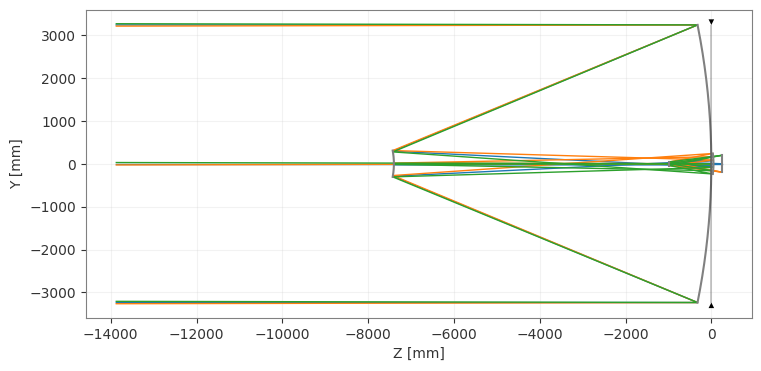
\includegraphics[width=\columnwidth]{figures/pearltma.png}
    \caption{Raytrace of the TMA model in Optiland. Multi-field PSF features used in inference are evaluated at ten field coordinates across the focal plane (see text).}
    \label{fig:pearltma}
\end{figure}

For each trial alignment vector $\boldsymbol{\theta}$, we build the TMA model and propagate the field with \bashinline{MMDFTPSF} using 512 rays, and retain a central $256\times256$ pixel intensity patch. The patch is projected onto the first 11 Zernike modes (Figure~\ref{fig:zernike_basis}), yielding an 11-element coefficient vector $\mathbf{c}_f(\boldsymbol{\theta})$ at each field point $f$. The synthetic observations $\mathbf{c}_{f,\mathrm{obs}}$ are computed from PSFs with additive Gaussian noise ($\sigma=0.01$ per pixel, in PSF intensity units), while forward-model PSFs in the likelihood are noise free. Nested sampling and differential evolution used separate noise realizations at the same $\sigma$, which has no practical effect on the nested-sampling stage (Section~\ref{sec:noise_likelihood}). Each covariance $\boldsymbol{\Sigma}_f$ is estimated from $10^4$ noise-free Monte Carlo draws with $\sigma=250\,\mu\mathrm{m}$ on $(pdx,pdy)$, $50\,\mu\mathrm{m}$ on $pdz$, $800\,\mu\mathrm{m}$ on $(sdx,sdy)$, $100\,\mu\mathrm{m}$ on $sdz$, $0.003$ degrees on $(ptx,pty)$, and $0.13$ degrees on $(stx,sty)$, with each draw rounded to two decimal places. The rounding sets about 90\% of the primary-tilt draws to exactly zero, but their standard deviation, $0.0031$ degrees, stays close to the intended value.

\begin{figure}
    \centering
    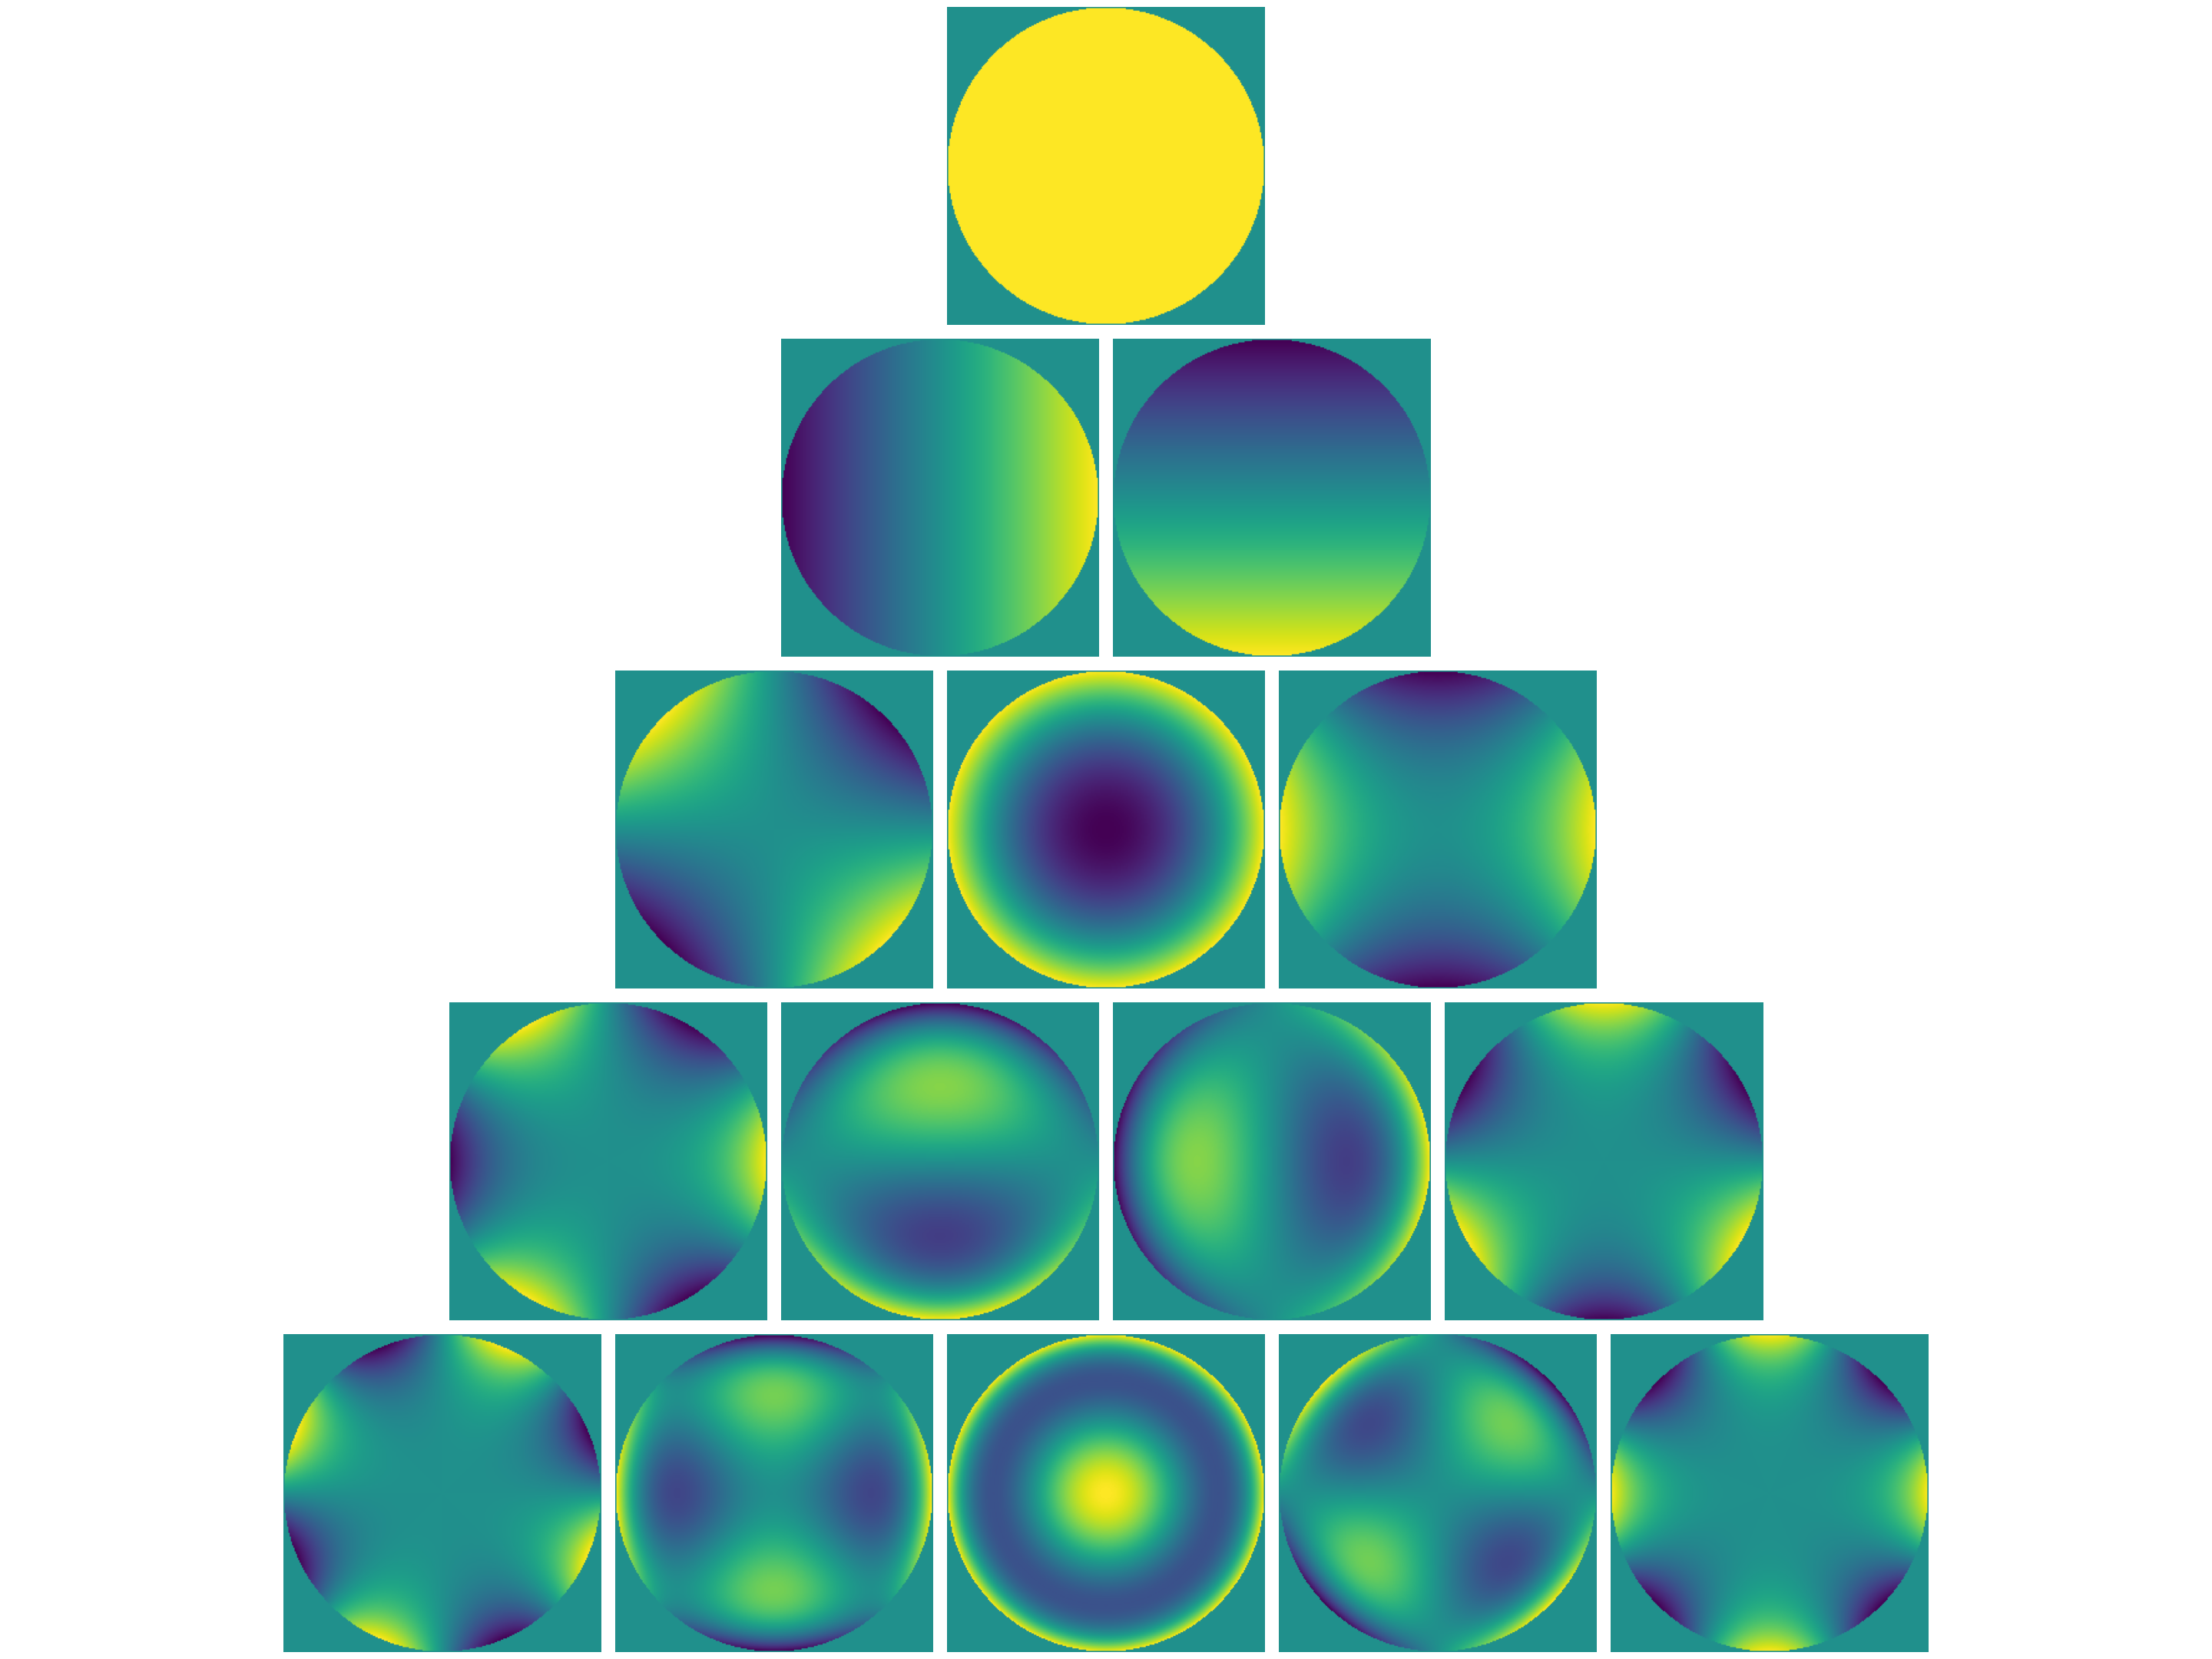
\includegraphics[width=0.75\textwidth]{figures/zernike_basis.png}
    \caption[The Zernike modes used for the TMA PSFs.]{The first 15 Zernike modes in Noll's ordering~\citep{Noll1976}, arranged as in Figure~\ref{fig:bessel_basis} so that each mode sits where its Fourier transform does. The modes are defined on the disk inscribed in the $256\times256$ image patch and are zero outside it. The TMA PSFs are projected onto the first 11: rows $n=0$--3 and primary spherical aberration at the center of the last row. Each panel has its own symmetric color scale, so zero has the same color in every panel.}
    \label{fig:zernike_basis}
\end{figure}

The prior transform maps uniform unit-cube samples to independent uniform boxes: primary decenters $(pdx,pdy)$ and despace $pdz \in [-800,800]\,\mu\mathrm{m}$, secondary decenters $(sdx,sdy)$ and despace $sdz \in [-2500,2500]\,\mu\mathrm{m}$, primary tilts $\in [-0.01,0.01]$ degrees, and secondary tilts $\in [-0.4,0.4]$ degrees. The weighted median $\mathbf{x}_0$ and the 2.1\%--97.9\% weighted quantiles of the final 100 posterior samples initialize and bound differential evolution. The DE objective is the unweighted sum of squared coefficient residuals over all ten fields, $\sum_{f\in\mathcal{F}}\sum_{k=1}^{11}[c_{f,k}(\boldsymbol{\theta})-c_{f,k,\mathrm{obs}}]^2$, minimized with \bashinline{tol=1e-10}; the run reached the limit of 2000 generations (final objective $2.2\times10^{-7}$) before L-BFGS-B polishing, which left the solution unchanged.

Recovered alignments $\mathbf{c}$ are validated by constructing a residual telescope with misalignments $(\boldsymbol{\theta}_{\mathrm{true}} - \mathbf{c})$ and comparing on-axis PSF images and OPD maps against the nominal system via \bashinline{OPD} at field $(0,0)$. We report both per-component residuals $\boldsymbol{\theta}_{\mathrm{true}} - \mathbf{c}$ and the RMS of the OPD difference in waves.

Both studies use Optiland for ray tracing, Nautilus for nested sampling, and SciPy~\citep{Virtanen2020} differential evolution for final refinement; the TMA study uses POPPY~\citep{Perrin2012} for the Zernike basis.

\section{Results}\label{sec:pearl_results}

The TMA study uses the noisy observations described in Sec.~\ref{sec:pearl}. Ten-dimensional nested sampling is computationally expensive; posterior medians need not coincide with injected truth when the likelihood contains flat directions. The posterior marginals in Figure~\ref{fig:pearl_corner} suggest partial degeneracies in the ten-dimensional problem. The primary decenter $pdx$ and both primary tilts are close to flat across their prior ranges, the secondary decenters remain broad, and several pairs are strongly correlated, notably $pdz$--$sdz$, $ptx$--$sdy$ and $pty$--$sdx$. The tilt--decenter correlations have a familiar optical origin: a tilt of one mirror about the $x$ ($y$) axis and a decenter of the other along $y$ ($x$) both introduce coma that is nearly constant across the field, so one can largely cancel the coma introduced by the other. The same mechanism made secondary-mirror misalignment on JWST detectable only through field-dependent aberrations (Chapter~\ref{sec:intro}): a compensating motion of another mirror cancels the field-constant error and leaves a field-dependent residual, which is why our likelihood combines several field points. The $pdz$--$sdz$ correlation similarly reflects the trade-off between the two despaces in setting focus. Only the secondary tilts are tightly constrained. Distinct alignment states may therefore produce similar Zernike vectors, and the likelihood alone may not determine every parameter uniquely.

\begin{figure*}
    \centering
    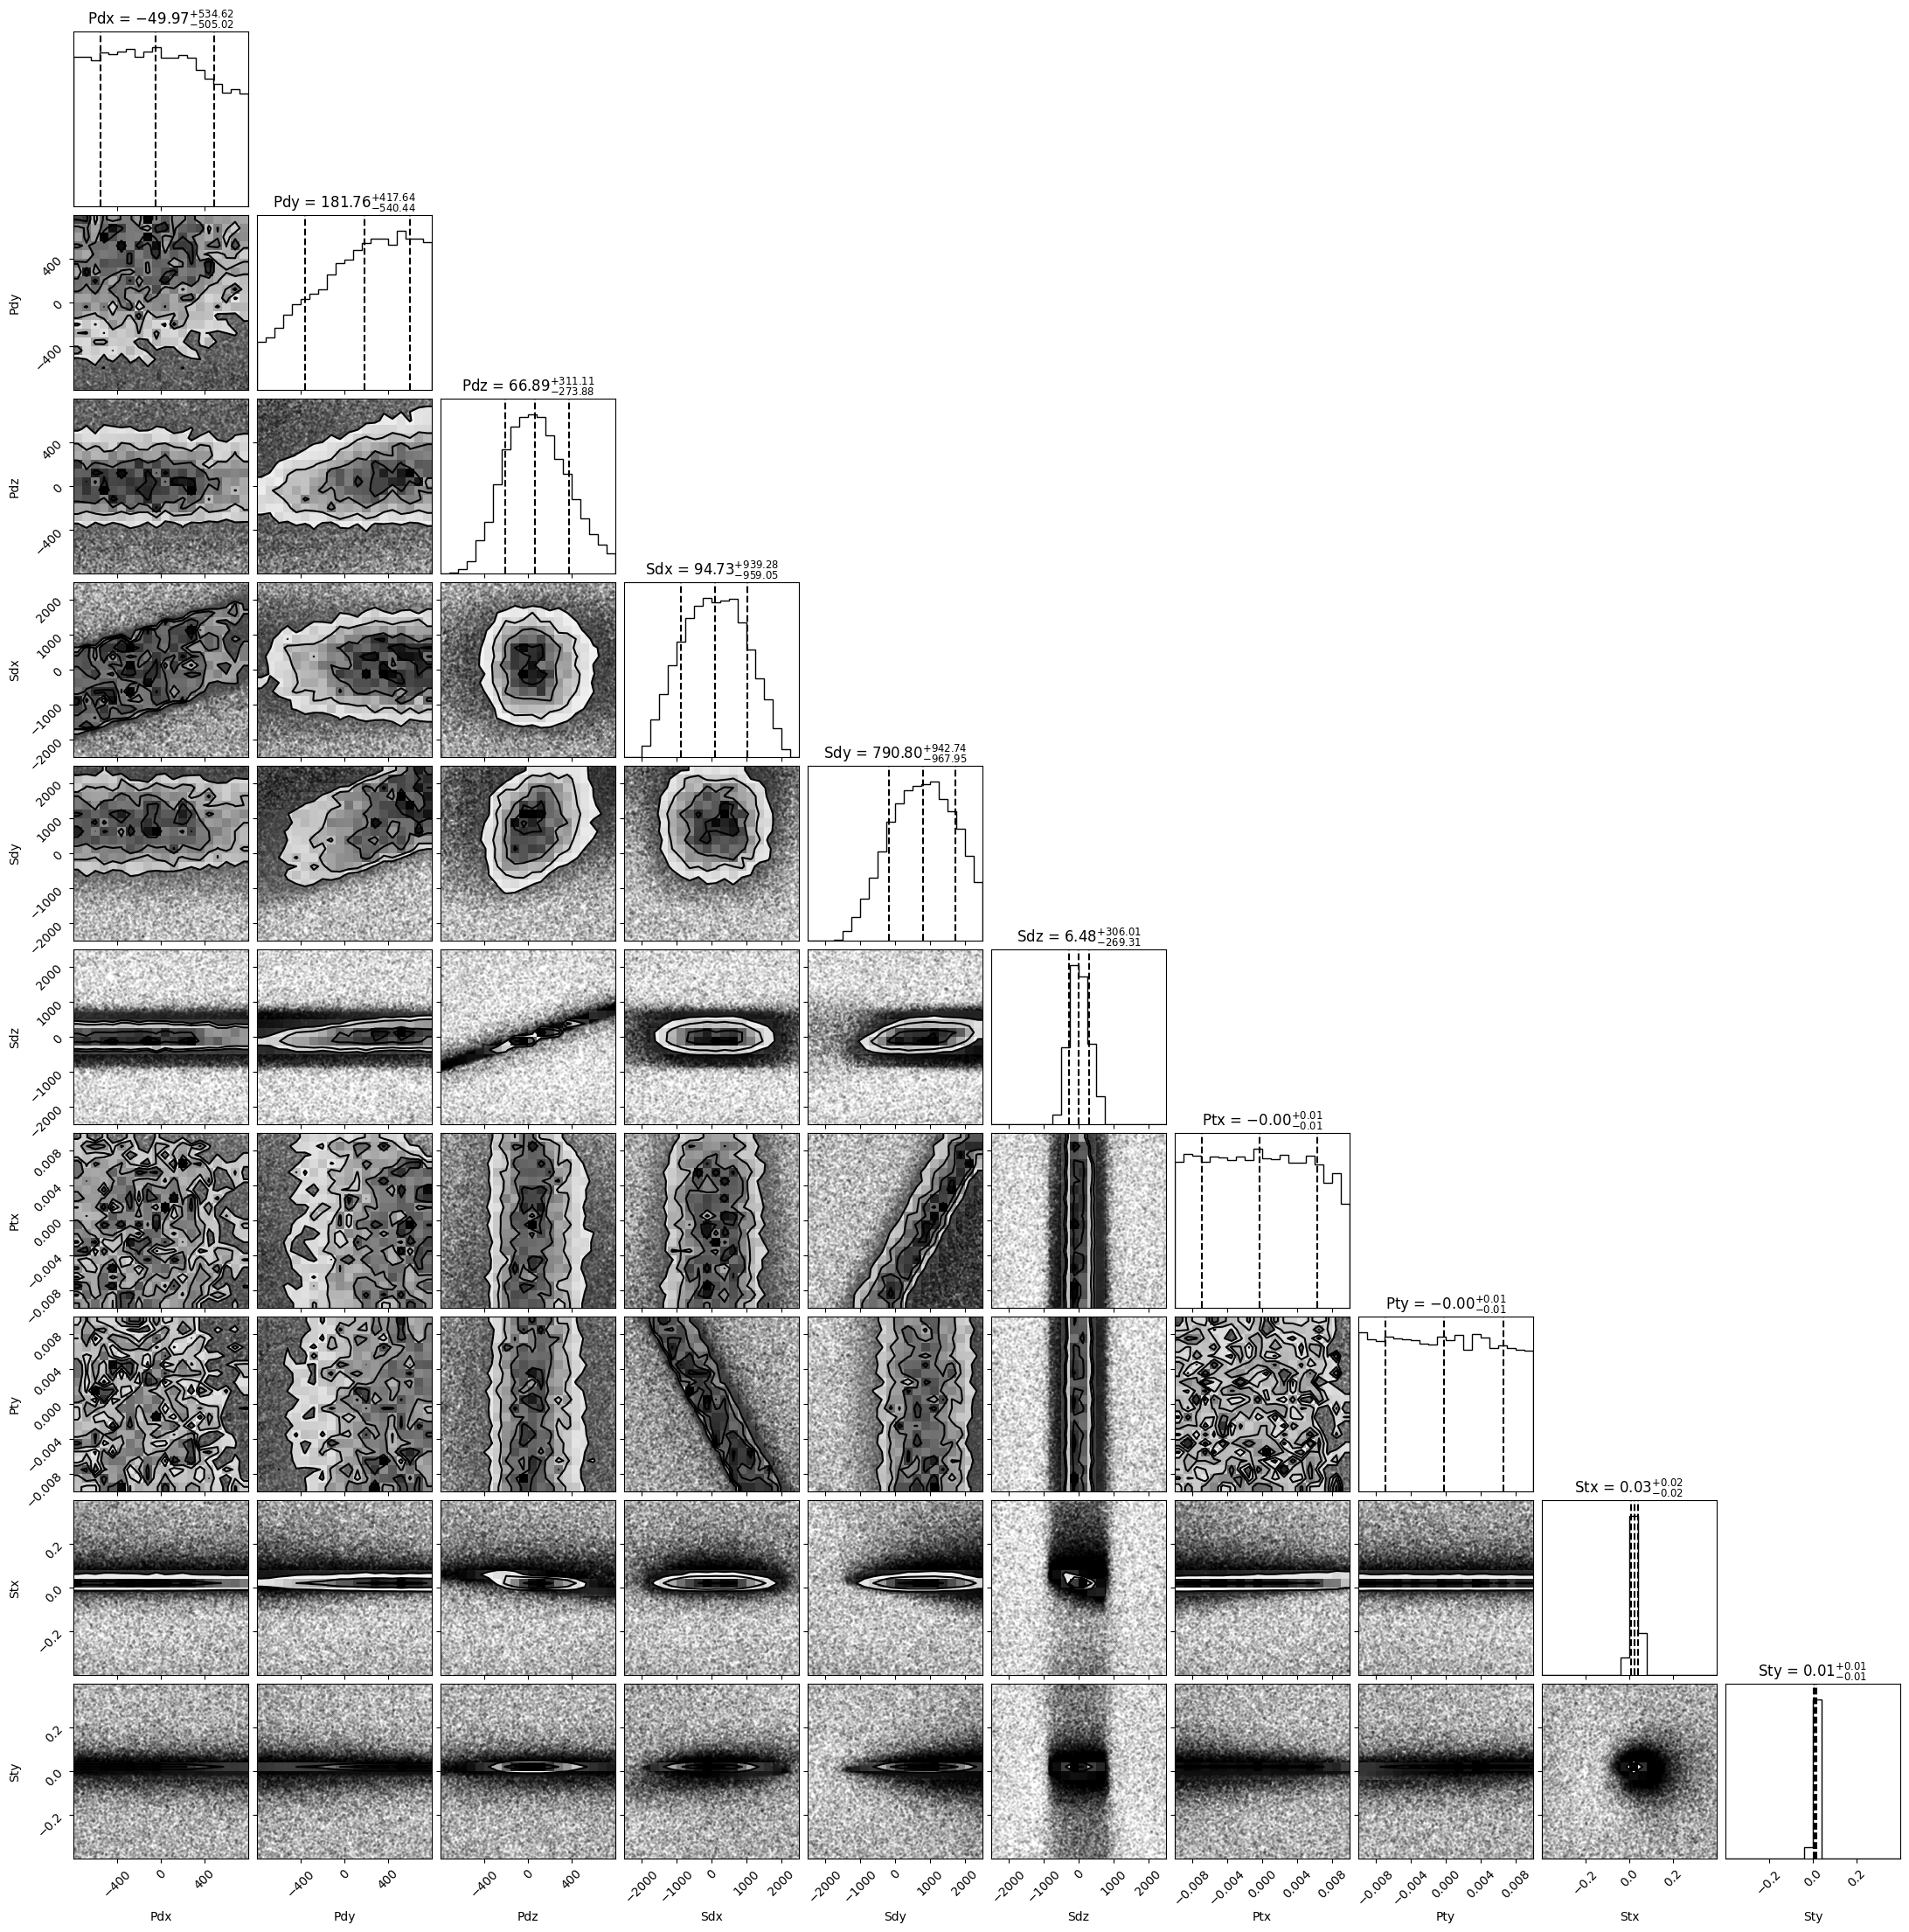
\includegraphics[width=\textwidth]{figures/pearltilus.png}
    \caption{Nautilus posterior corner plot for the ten primary/secondary misalignment parameters of the TMA model.}
    \label{fig:pearl_corner}
\end{figure*}

Nautilus performed 93\,200 likelihood evaluations with $\ln\mathcal{Z}\approx +475.5$ and $N_{\mathrm{eff}}\approx 2.04\times 10^4$. With no correction, on-axis OPD RMS is $\sim 8.24$ waves, and the DE starting point $\mathbf{x}_0$ (the median of the final 100 posterior samples) alone reduces this to $\sim 0.99$ waves. Table~\ref{tab:pearl} reports the truth and DE-refined alignment states: the refinement reduces on-axis OPD RMS to $\sim 2.5\times 10^{-3}$ waves while leaving residuals of up to $\sim 46\,\mu\mathrm{m}$ on the translations (largest on secondary decenter $sdx$; the other translations are within $10.3\,\mu\mathrm{m}$). Primary tilts are near zero at truth and remain poorly determined relative to translations. Figure~\ref{fig:tma_psf_prog} shows the on-axis PSF and RMS wavefront error at each stage of the refinement, and Figure~\ref{fig:tma_opd} the residual OPD maps. As for Hubble, the final residual is dominated by low-order terms, tilt (66\% of the variance) and defocus (26\%).

\begin{table}
\centering
\caption[TMA: injected truth and DE-recovered alignment.]{TMA: injected truth and DE-recovered alignment (after 2000 generations and L-BFGS-B polishing).}
\label{tab:pearl}
\begin{tabular}{llll}
\hline
\textbf{Parameter} & \textbf{True value} & \textbf{Recovered} & \textbf{Units} \\
\hline
pdx  & $-152.75$ & $-155.30$ & $\mu$m \\
pdy  & $316.91$  & $327.15$  & $\mu$m \\
pdz  & $26.63$   & $30.26$   & $\mu$m \\
sdx  & $-42.31$  & $3.81$    & $\mu$m \\
sdy  & $923.33$  & $932.86$  & $\mu$m \\
sdz  & $-32.75$  & $-29.22$  & $\mu$m \\
ptx  & $2.98\times 10^{-5}$ & $6.71\times 10^{-6}$ & degree \\
pty  & $1.61\times 10^{-5}$ & $-3.50\times 10^{-4}$  & degree \\
stx  & $0.0269$  & $0.0268$  & degree \\
sty  & $0.0098$  & $0.0095$  & degree \\
\hline
\end{tabular}
\end{table}

\begin{figure*}
    \centering
    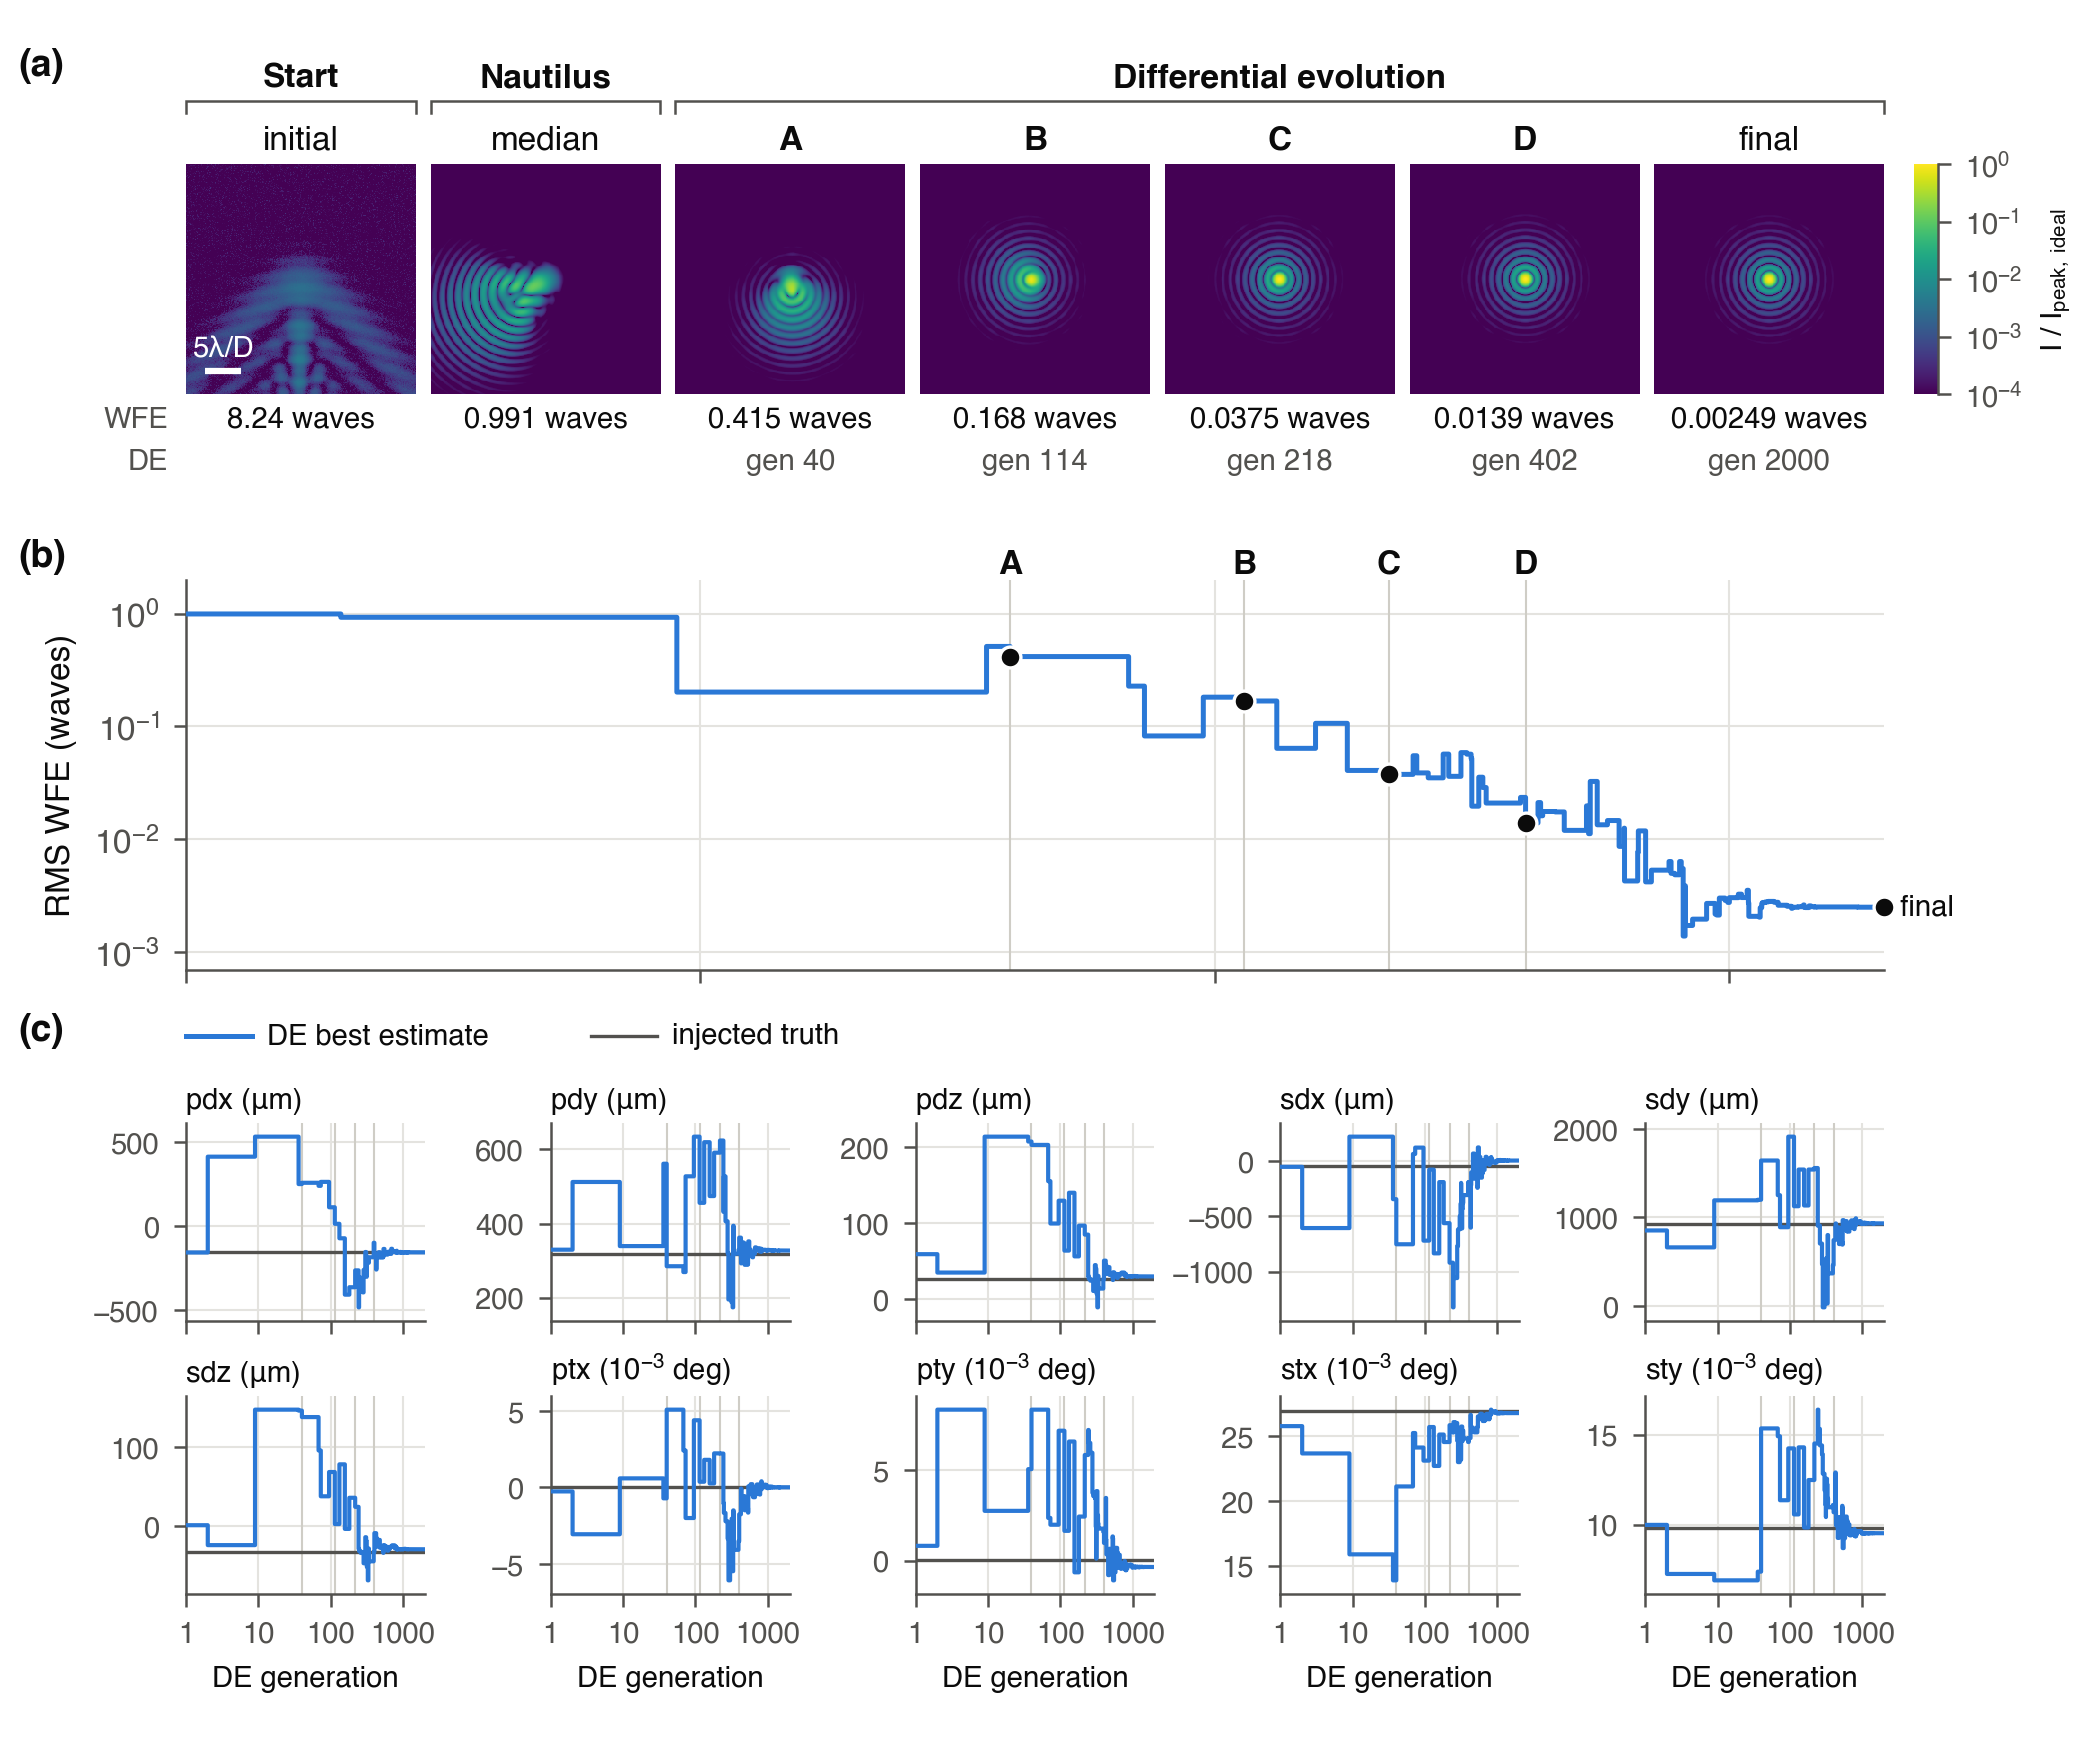
\includegraphics[width=\textwidth]{figures/tma_psf_progression.png}
    \caption{TMA benchmark: (a) On-axis PSFs at $\lambda = 0.65\,\mu\mathrm{m}$: the observed misaligned PSF (Gaussian noise, $\sigma = 0.01\%$ of the ideal peak), the Nautilus starting point (median of the final 100 posterior samples), during differential evolution (DE) at generations 40, 114, 218 and 402 (A--D), and after 2000 generations (final). Intensity is relative to the aligned system's peak, so each panel's peak equals its Strehl ratio (log stretch, floor $10^{-4}$). Values are RMS wavefront error in waves, the RMS of the OPD difference from the nominal design. (b) RMS WFE of the best DE member at each generation; letters mark the PSFs in (a). (c) Best-member value of each alignment parameter at each generation (blue) and the injected truth (gray).}
    \label{fig:tma_psf_prog}
\end{figure*}

\begin{figure*}
    \centering
    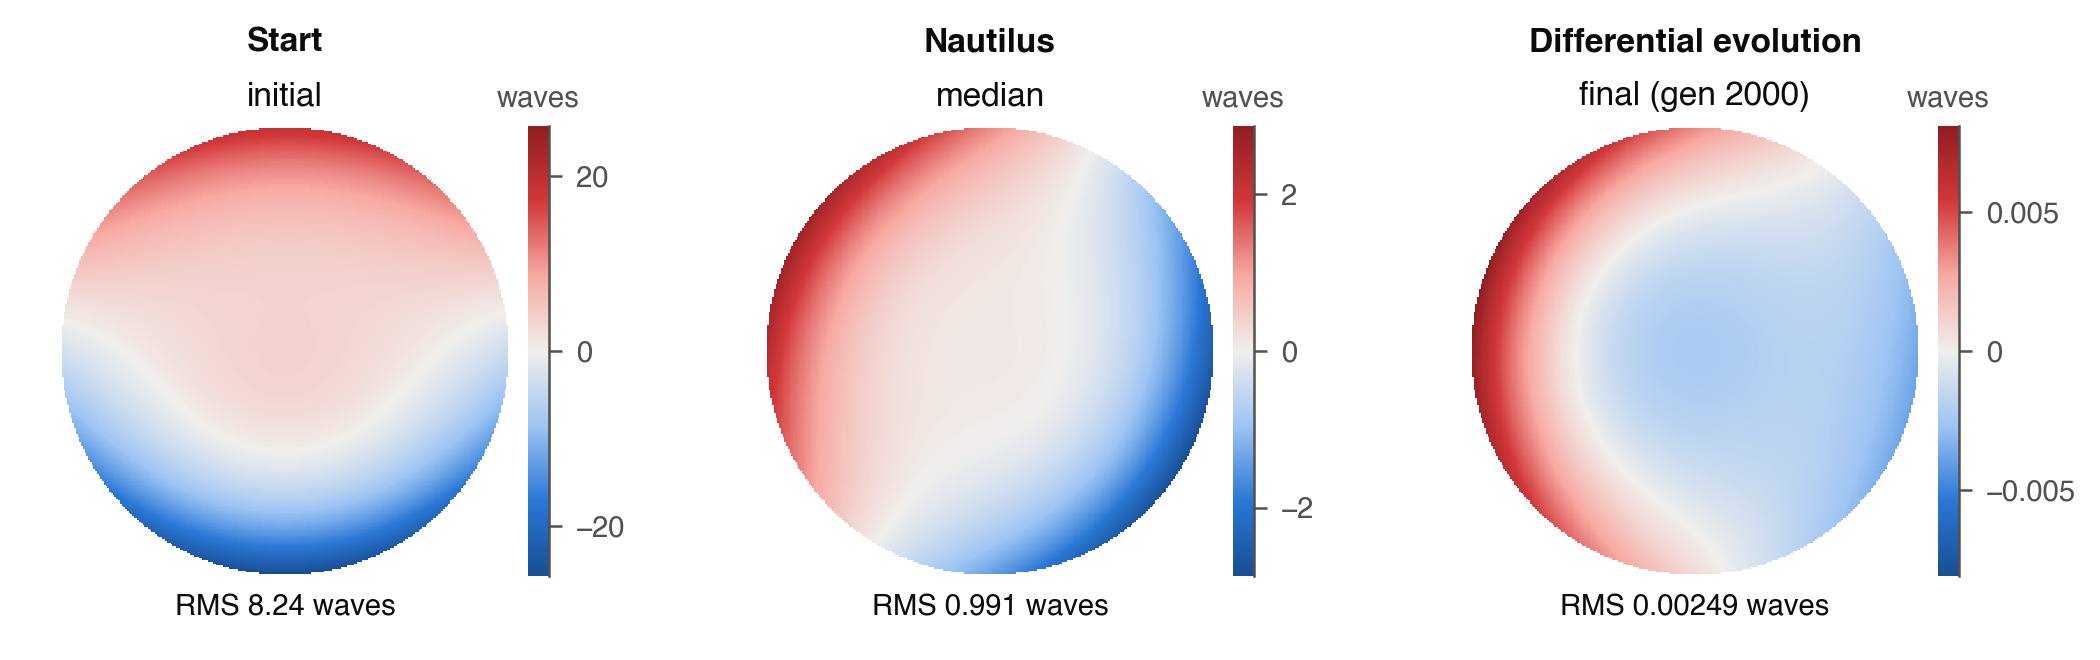
\includegraphics[width=\textwidth]{figures/tma_opd.png}
    \caption{Residual on-axis OPD maps of the TMA: the difference between the nominal design and the system with residual misalignment $\boldsymbol{\theta}_{\mathrm{true}}-\mathbf{c}$, for the uncorrected system, the Nautilus starting point and the DE solution after 2000 generations and L-BFGS-B polishing. Piston is removed and tilt is retained, as in the quoted RMS WFE. Each panel has its own symmetric color scale in waves, with zero in gray. By variance, the final residual is 66\% tilt and 26\% defocus.}
    \label{fig:tma_opd}
\end{figure*}